\documentclass[a4paper,10pt]{beamer}
\usepackage[utf8]{inputenc}
\usepackage{color}
\usepackage{colortbl}
\usepackage{xcolor}
\usepackage{tikz}
\usepackage{caption}
\usepackage{ragged2e}
\renewcommand{\figurename}{Figura}
\usetheme{Madrid} % Ver https://deic.uab.cat/~iblanes/beamer_gallery/index_by_theme.html
\useoutertheme{miniframes} % Alternatively: miniframes, infolines, split
\useinnertheme{circles}

\AtBeginSection[]{
  \begin{frame}
  \vfill
  \centering
  \begin{beamercolorbox}[sep=8pt,center,shadow=true,rounded=true]{title}
    \usebeamerfont{title}\insertsectionhead\par%
  \end{beamercolorbox}
  \vfill
  \end{frame}
}

%\definecolor{UBCblue}{rgb}{0.04706, 0.13725, 0.26667} % UBC Blue (primary)
%\usecolortheme[named=UBCblue]{structure}
%\usecolortheme[named=Mahogany]{structure} % Sample dvipsnames color

\title{Métodos numéricos de resolución de sistemas no lineales}
\author{Milagrosa Sánchez Carrero}
\date{}

% !TEX program = pdflatex

\begin{document}

\begin{frame}
	\maketitle
\end{frame}

% \frame{
% 	\Large{Índice}
% 	\tableofcontents
% }

\section{Introducción}
\begin{frame}{Introducción}

\begin{itemize}
	\item En el primer capítulo desarrollaremos los métodos directos, como son el \textbf{método del punto fijo}, el \textbf{método de Newton} y los \textbf{métodos cuasi-Newton}. Estos métodos generan una sucesión de estimaciones que convergen a la solución.
	\pause
	\item En el segundo capítulo, hablaremos del \textbf{método de máximo descenso} y su alternativa, el \textbf{método del gradiente conjugado}. Estos métodos pretenden la resolución de sistemas transformándolos en un problema equivalente de cálculo de mínimos absolutos para nuestra función.
	\pause
	\item El tercer capítulo tratará de los \textbf{métodos de continuación homotópica}. Estos métodos crean una homotopía entre el problema original y un problema trivial, para ajustar progresivamente una solución del problema trivial a la solución buscada.
\end{itemize}
\end{frame}

\section{Métodos directos}

\begin{frame}
	\begin{itemize}
		\item Nos interesaremos por sistemas de ecuaciones de la forma:
		\[
			\begin{cases}
				f_1(x_1,\dots,x_n)  = 0 \\
				f_2(x_1,\dots,x_n)  = 0 \nonumber \\
				...                   \nonumber \\
				f_n(x_1,\dots,x_n)  = 0 \nonumber
			\end{cases}
		\]
		\pause
		\item Esto equivale a buscar ceros de una función $F : \mathbb{R}^n \to \mathbb{R}^n$
	\end{itemize}
\end{frame}

\subsection{Método del punto fijo}
\begin{frame}{Método del punto fijo}

\begin{itemize}
	\item Se basa en reformular el problema original en un un problema de búsqueda de un punto fijo $G(x)=x$.
	\pause
	\item Es eficiente para encontrar soluciones precisas en un número finito de iteraciones.
	\pause
	\item Sin embargo, la convergencia del método dependerá de las propiedades de la función elegida $G$.
\end{itemize}
\end{frame}

\begin{frame}{Método del punto fijo}
	\begin{itemize}
		\item Transformamos algebraicamente $F(x)=0$ en un problema de punto fijo $G(x)=x$.
		\item Se toma una aproximación inicial $x_0$.
		\item Para cada $k\geq 0$:
		\begin{itemize}
			\item Se toma $x_{k+1} = G(x_k)$.
			\item El proceso se repite hasta que se alcanza un criterio de convergencia, como un número máximo de iteraciones o una tolerancia de error predefinida.
		\end{itemize}
	\end{itemize}
\end{frame}

\subsection{Método de Newton}
\begin{frame}{Método de Newton}

	\begin{itemize}
\item En una dimensión, se basa en la idea de aproximar la función por una recta tangente en cada iteración. Se generaliza en varias dimensiones usando el jacobiano.
\pause
\item Converge cuadráticamente hacia la raíz cuando se cumplen ciertas condiciones de continuidad.
\pause
\item Sin embargo, puede ser sensible a la elección de la aproximación inicial y puede no converger en algunos casos.
	\end{itemize}
\end{frame}

\begin{frame}{Método de Newton}
	\begin{itemize}
		\item El proceso comienza con la elección de una aproximación inicial $x_0$.
		\item En cada iteración $k$, se toma como la siguiente aproximación 
		\begin{equation*}
			x_{k+1} = x_{k} + J(x_{k})^{-1}(-F(x_k)) \onslide<2->{\textcolor{red}{ =G(x_k)}}
		\end{equation*}
		\item El proceso se repite hasta que se alcanza un criterio de convergencia, como un número máximo de iteraciones o una tolerancia de error predefinida.	
	\end{itemize}

\end{frame}

\begin{frame}{Método de Newton: Limitaciones}
	\begin{block}{Limitaciones}
		La matriz Jacobiana puede ser costosa de calcular en algunos casos.
	\end{block}
	
	Esto motiva los métodos cuasi-Newton.
\end{frame}

\subsection{Métodos cuasi-Newton}
\begin{frame}{Métodos cuasi-Newton}

\begin{itemize}
	\item Los métodos cuasi-Newton son variantes del método de Newton especialmente útiles cuando la matriz Jacobiana es costosa de calcular o no está disponible analíticamente. En su lugar, se usan aproximaciones de la matriz Jacobiana.
	\pause
	\item Permiten reducir el número de evaluaciones y cálculos necesarios en comparación con el método de Newton original. Pero pueden introducir errores en la precisión de la solución.
	\pause
	\item Veremos como ejemplo el método de Broyden.
\end{itemize}

\end{frame}

\begin{frame}{Método de Broyden}
	\begin{itemize}
		\item Estimar el jacobiano por:
	\begin{equation}\label{SM}
		A_i = A_{i-1} + \frac{y_i-A_{i-1} s_i}{||s_i||^2_2}s^t_i
	\end{equation}
	
	donde $y_i = x_i-A_i^{-1}F(x_{i})$ y $s_i = x_{i} - x_{i-1}$.

		\item Usar el método de Newton con la estimación:
		
	\[x_{i+1} = x_{i}-A_i^{-1} F(x_{i})\]
	
\end{itemize}
\end{frame}

\begin{frame}{Método de Broyden: Limitaciones}

	\begin{block}{Limitaciones}
	Cálculo de una matriz inversa distinta en cada paso.
	\end{block}
	\pause

	Pero esto se puede evitar usando la fórmula de Sherman-Morrison.
	
\[A^{-1}_i = A_{i-1}^{-1} - \frac{(	A_{i-1}^{-1} y_{i} - s_{i}) s_{i}^{t} 	A_{i-1}^{-1}  }{ ||s_{i}||_2^2 + s_{i}^{t} A_{i-1}^{-1} y_{i} - ||s_{i}||_2^2 } \]
\end{frame}

\section{Optimización sin restricciones}

\begin{frame}
	\begin{itemize}
		\item En esta sección, exploramos métodos de minimización de funciones no lineales $f : \mathbb{R}^n\to\mathbb{R}$.
		\pause
		\item El problema de encontrar soluciones de una ecuación $F(x)=b$ se puede reescribir como el problema de minimizar $\|F(x)-b\|^2$.
	\end{itemize}
\end{frame}

\subsection{Método del máximo descenso}
\begin{frame}{Método del máximo descenso}

\begin{itemize}
	\item Se basa en la idea de seguir la \textbf{dirección de máximo descenso} (la dirección opuesta al gradiente) de la función en cada iteración.
	\pause
	\item La tasa de aprendizaje (es decir, la elección tamaño del paso) en cada iteración se hace por algún algoritmo de búsqueda lineal, como \textbf{backtracking}.
	\pause
	\item Puede ser sensible a la elección del punto inicial y puede converger lentamente en algunos casos
\end{itemize}

\end{frame}

\begin{frame}{Método del máximo descenso}
	\begin{itemize}
		\item El proceso comienza con la elección de una estimación inicial $x_0$.
		\item En cada iteración $k$ se calcula la tasa de aprendizaje $L_k$ y se calcula la siguiente aproximación:
			\[ x_{k+1} = x_{k} - L_k \nabla f(x_k) \]
		\item Se interrumpen las iteraciones si $\nabla f(x_k)$ es muy pequeño.
	\end{itemize}
\end{frame}

\begin{frame}{Método del máximo descenso: Backtracking}
	\begin{itemize}
		\item Si para el cálculo de la tasa de aprendizaje se usa \textit{backtracking}, basta tomar un paso suficientemente pequeño para que se cumpla la \textbf{condición de Armijo}:
		\[ f(x-t \nabla f(x)) \leq f(x) - \gamma t \|\nabla f(x)\|_2^2 \]
	\end{itemize}
\end{frame}

\subsection{Método del gradiente conjugado}
\begin{frame}{Método del gradiente conjugado}

\begin{itemize}
	\item El método gradiente conjugado es similar al método del máximo descenso.
	\pause
	\item Se basa en la idea de buscar una dirección conjugada respecto al Hessiano en cada iteración.
\end{itemize}
\end{frame}

\begin{frame}{Método del gradiente conjugado: Algoritmo}

	\begin{itemize}
		\item Tomar una estimación inicial $x_0$ y una dirección de descenso inicial $p_0=-\nabla f(x_0)$ y un residuo inicial $r_0=p_0$.
		\item Para cada $k$ mientras $r_{k}$ sea grande:
		\begin{itemize}
			\item Calcular $a_k$ que minimiza $f(x_k + a_k p_k)$ con búsqueda lineal.
			\item Tomar nueva estimación $x_{k+1} = x_k + a_k p_k$.
			\item Tomar nuevo residuo $r_{k+1} = - \nabla f(x_{k+1})$.
			\item Calcular $\beta_{k+1}$ y actualizar $p_{k+1} = \beta_{k+1} p_k - \nabla f(x_{k+1})$.
		\end{itemize}
		\pause
		\item Hay varias posibilidades para el cálculo de $\beta_k$:
		\begin{itemize}
		\item Fletcher-Reeves:
		\[\beta_{k+1}^{FR} = \frac{r^t_{k+1} r_{k+1}}{r^t_k r_k} = \frac{\|r_{k+1}\|^2}{\|r_k\|^2} = \frac{\|f'(x_{k+1})\|^2}{\|f'(x_k)\|^2} \]
		\item Polak-Rivière:
		\[\beta_{k+1}^{PR} = \frac{r^t_{k+1} (r_{k+1}-r_k)}{r^t_k r_k} \]
		\end{itemize}
	\end{itemize}
\end{frame}

\begin{frame}{Ejemplo: Método máximo descenso y gradiente conjugado}
	\[ f(x,y) = x^4 - 2x^2y + x^2+ y^2-2x + 1 \]


	\begin{center}
	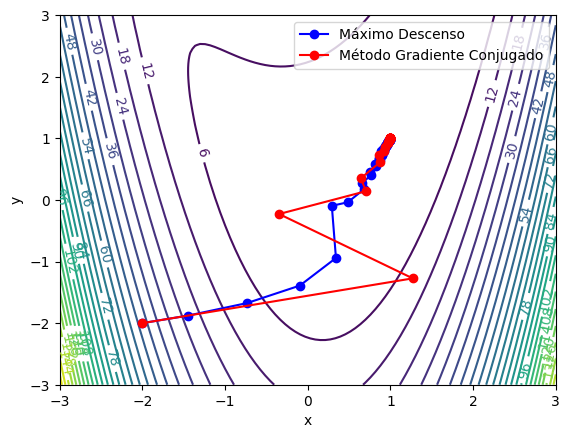
\includegraphics[scale=0.5]{metodos.png}
	\end{center}
\end{frame}
\section{Método de continuación homotópica}
\begin{frame}{Método de continuación homotópica}

\begin{itemize}
	
	\item Se basa en la idea de deformar continuamente una función inicial $f_0$ fácil de resolver hacia la función objetivo $f$ utilizando una homotopía $H(x,\lambda)$ de $f_0$ a $f$.
	\pause
	\item La homotopía forma una curva $H(x,\lambda)=0$ de soluciones, donde $H(x,1)=0$ son las soluciones que buscamos.
	\pause
	\item Estos métodos son útiles cuando se tiene información limitada sobre la solución deseada, incluso cuando no se tiene una aproximación inicial cercana a la solución exacta.
	\pause
	\item Además, se pueden usar el mismo método para encontrar simultáneamente varias soluciones del problema.
	\pause
	\item Existen diferentes variantes de los métodos de continuación homotópica, en el trabajo estudiamos el método de continuación homotópica de Euler-Newton que es un \textbf{método predictor-corrector}.
\end{itemize}

\end{frame}

\begin{frame}{Método de continuación homotópica de Euler-Newton}

	\begin{itemize}
		\item En la forma de Euler-Newton, se usa el método de Euler para estimar el valor de la solución y el método de Newton para corregirlo.
		\item En cada paso, se usa la solución anterior como estimación inicial para el nuevo problema a lo largo de la curva $H(x,\lambda)=0$.
		\begin{figure}[H]
			\centering
		
			\tikzset{every picture/.style={line width=0.75pt}} %set default line width to 0.75pt        
		
			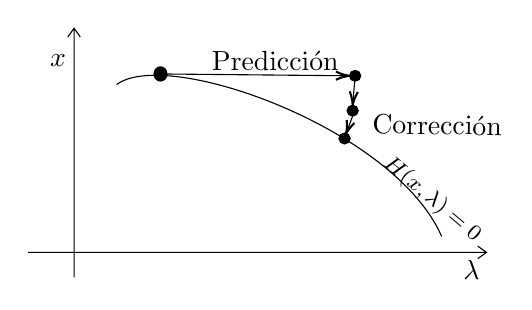
\begin{tikzpicture}[x=0.75pt,y=0.75pt,yscale=-0.6,xscale=0.6]
			%uncomment if require: \path (0,300); %set diagram left start at 0, and has height of 300
			
			%Curve Lines [id:da3653140690727089] 
			\draw    (102.6,130.78) .. controls (142.6,100.78) and (325.6,165.78) .. (363.6,252.78) ;
			%Flowchart: Connector [id:dp392125415090699] 
			\draw  [fill={rgb, 255:red, 0; green, 0; blue, 0 }  ,fill opacity=1 ] (132.6,122.29) .. controls (132.6,119.13) and (134.93,116.58) .. (137.8,116.58) .. controls (140.68,116.58) and (143,119.13) .. (143,122.29) .. controls (143,125.44) and (140.68,127.99) .. (137.8,127.99) .. controls (134.93,127.99) and (132.6,125.44) .. (132.6,122.29) -- cycle ;
			%Straight Lines [id:da32974900830101495] 
			\draw    (137.8,122.29) -- (215.6,123.05) -- (287.6,123.76) ;
			\draw [shift={(289.6,123.78)}, rotate = 180.57] [color={rgb, 255:red, 0; green, 0; blue, 0 }  ][line width=0.75]    (10.93,-3.29) .. controls (6.95,-1.4) and (3.31,-0.3) .. (0,0) .. controls (3.31,0.3) and (6.95,1.4) .. (10.93,3.29)   ;
			%Flowchart: Connector [id:dp396415556899567] 
			\draw  [fill={rgb, 255:red, 0; green, 0; blue, 0 }  ,fill opacity=1 ] (289.6,123.78) .. controls (289.6,121.38) and (291.61,119.43) .. (294.1,119.43) .. controls (296.59,119.43) and (298.6,121.38) .. (298.6,123.78) .. controls (298.6,126.19) and (296.59,128.14) .. (294.1,128.14) .. controls (291.61,128.14) and (289.6,126.19) .. (289.6,123.78) -- cycle ;
			%Flowchart: Connector [id:dp8330801591176681] 
			\draw  [fill={rgb, 255:red, 0; green, 0; blue, 0 }  ,fill opacity=1 ] (287.6,151.78) .. controls (287.6,149.38) and (289.61,147.43) .. (292.1,147.43) .. controls (294.59,147.43) and (296.6,149.38) .. (296.6,151.78) .. controls (296.6,154.19) and (294.59,156.14) .. (292.1,156.14) .. controls (289.61,156.14) and (287.6,154.19) .. (287.6,151.78) -- cycle ;
			%Flowchart: Connector [id:dp25418827796224785] 
			\draw  [fill={rgb, 255:red, 0; green, 0; blue, 0 }  ,fill opacity=1 ] (281.1,174.14) .. controls (281.1,171.73) and (283.11,169.78) .. (285.6,169.78) .. controls (288.09,169.78) and (290.1,171.73) .. (290.1,174.14) .. controls (290.1,176.54) and (288.09,178.49) .. (285.6,178.49) .. controls (283.11,178.49) and (281.1,176.54) .. (281.1,174.14) -- cycle ;
			%Straight Lines [id:da9516946974155029] 
			\draw    (294.1,123.78) -- (293.08,135.82) -- (292.27,145.44) ;
			\draw [shift={(292.1,147.43)}, rotate = 274.83] [color={rgb, 255:red, 0; green, 0; blue, 0 }  ][line width=0.75]    (10.93,-3.29) .. controls (6.95,-1.4) and (3.31,-0.3) .. (0,0) .. controls (3.31,0.3) and (6.95,1.4) .. (10.93,3.29)   ;
			%Straight Lines [id:da17213986288020022] 
			\draw    (292.1,156.14) -- (287.3,168.91) ;
			\draw [shift={(286.6,170.78)}, rotate = 290.58] [color={rgb, 255:red, 0; green, 0; blue, 0 }  ][line width=0.75]    (10.93,-3.29) .. controls (6.95,-1.4) and (3.31,-0.3) .. (0,0) .. controls (3.31,0.3) and (6.95,1.4) .. (10.93,3.29)   ;
			%Shape: Axis 2D [id:dp7268441229557736] 
			\draw  (31.6,265.58) -- (399.6,265.58)(68.4,85.58) -- (68.4,285.58) (392.6,260.58) -- (399.6,265.58) -- (392.6,270.58) (63.4,92.58) -- (68.4,85.58) -- (73.4,92.58)  ;
			
			% Text Node
			\draw (177,102) node [anchor=north west][inner sep=0.75pt]   [align=left] {Predicción};
			% Text Node
			\draw (306.13,152.56) node [anchor=north west][inner sep=0.75pt]  [rotate=-0.88] [align=left] {Corrección};
			% Text Node
			\draw (379,270) node [anchor=north west][inner sep=0.75pt]   [align=left] {$\displaystyle \lambda $};
			% Text Node
			\draw (47,104.4) node [anchor=north west][inner sep=0.75pt]    {$x$};
			% Text Node
			\draw (324.66,182.45) node [anchor=north west][inner sep=0.75pt]  [font=\footnotesize,rotate=-40.12]  {$H( x,\lambda ) =0$};
			
			\end{tikzpicture}	
		\end{figure}
	\end{itemize}
\end{frame}

\begin{frame}{Método de continuación homotópica de Euler-Newton}
	\begin{itemize}
		\item Se toma una función inicial $f_0$ con raíz $x_0$ y una homotopía $H$ de $f_0$ a $f$.
		\item En cada paso $k$ hasta convergencia:
		\begin{itemize}
			\item Predictor: $x_{k+1}' = x_k + h H'(x_k)$.
			\item Corrector: Se calcula $x_{k+1}$ con el método de Newton usando $x_{k+1}'$ como estimación inicial.
		\end{itemize}
	\end{itemize}
	
\end{frame}

\appendix

\begin{frame}
	\vfill
	\centering
	\begin{beamercolorbox}[sep=8pt,center,shadow=true,rounded=true]{title}
		\usebeamerfont{title}Gracias por su atención\par%
	\end{beamercolorbox}
	\vfill
\end{frame}
\end{document}